\section{DeEmbed User Guide}
This section will walk you through the usage of DeEmbed, we will show which files can be loaded and how to use calibration files. Also the navigation through the chart will be explained shortly.
\subsection{Loading Calibration files}
\label{sec:loadingcalfiles}
In order to deembed the actual S-Parameters $S$ from the measured S-Parameters $S_M$, you need to supply the measured (or simulated) calibration files for Short, Open, Load, Through and Isolation. 
\begin{figure}[H]
	\centering
	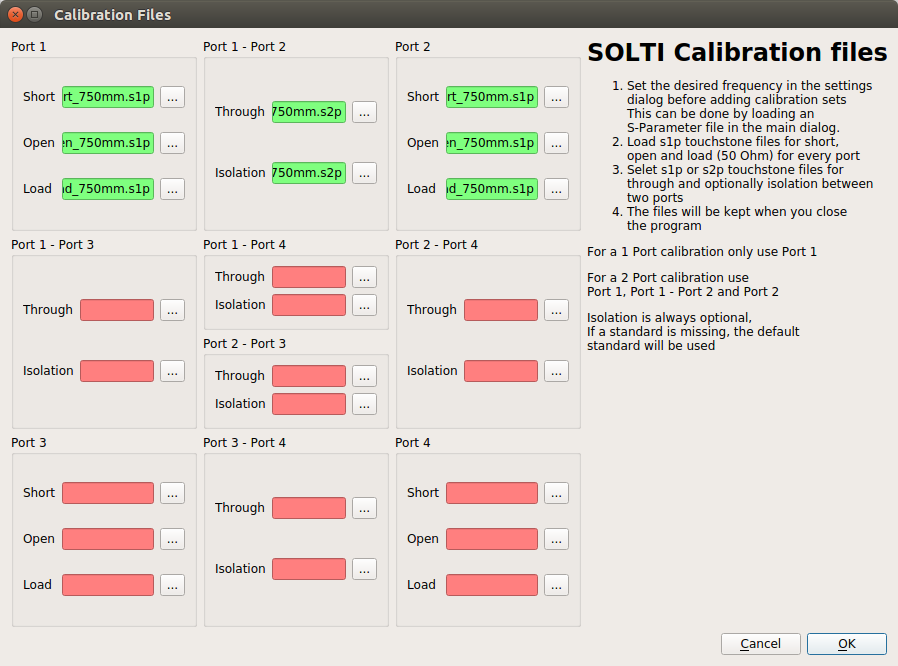
\includegraphics[width=0.75\textwidth]{figures/screenshot3.png}
	\caption{Calibration files dialog}
	\label{fig:caldialog}
\end{figure}
Figure \ref{fig:caldialog} shows the dialog in which the filenames of the measured calibration standards are specified. Depending on the number of ports of the DUT (Device under Test) a number of TouchStone files with measured standards must be supplied. For every port, the following files must be present:
\begin{itemize}
	\item {\textbf{Short:} A measured trace with an uncalibrated network analyzer of the short standard. The file is a one port Touchstone file (.s1p) }
	\item {\textbf{Open:} A measured trace with an uncalibrated network analyzer of the open standard. The file is a one port Touchstone file (.s1p) }
	\item {\textbf{Load:} A measured trace with an uncalibrated network analyzer of the $50\Omega$ load standard. The file is a one port Touchstone file (.s1p) }

\end{itemize}
If the DUT consists of more than one port, also through and optionally isolation standards should be supplied. 
\begin{itemize}
	\item {\textbf{Through:} A measured trace with an uncalibrated network analyzer between the two corresponding ports, with the two cables connected together with a through connector. The file is a two port Touchstone file (.s2p)}
	\item {\textbf{Through:} A measured trace with an uncalibrated network analyzer between the two corresponding ports, with the two cables both connected to a $50\Omega$ load. The file is a two port Touchstone file (.s2p)}
\end{itemize}
The format of the Touchstone files is described in \cite{touchstoneformat}.

If you want to de-embed a two port S-Parameter file, only Short, Open and Load for Port 1 and 2 need to be supplied plus the Through and Isolation between Port 1-2, this calibration set is shown in figure \ref{fig:caldialog}.

If the file supplied with the browse button (...) can be found, the filename colors green, otherwise the box turns red. The green color does not indicate that the file is a valid Touchstone file.

\subsection{Setting calibration standards}
\label{sec:settingcalstds}

The measured calibration standards described in \ref{sec:loadingcalfiles} are usually not measured with perfect calibration standards, unless a simulator is used to generate the calibration files. In case of a perfect calibration kit, the calibration set ''Ideal''can be used.

\begin{figure}[H]
	\centering
	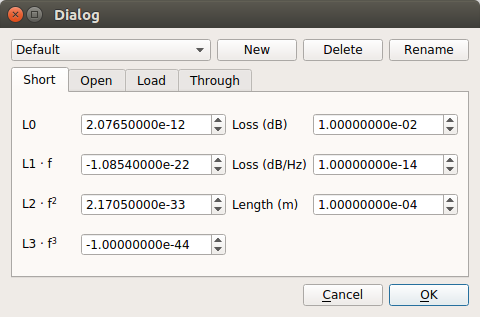
\includegraphics[width=0.75\textwidth]{figures/screenshot4.png}
	\caption{Calibration standards dialog}
	\label{fig:calstddialog}
\end{figure}
\subsection{Open and save Touchstone files}
\subsection{Navigate the chart}
\newpage
